\chapter{Versionsverwaltung}\label{cha:Versionsverwaltung}
\section{Definition}\label{sec:Definition}
Versionsverwaltungssysteme sind auch bekannt als Versionskontrollsysteme
(\acrlong{vcs}), Quellcode Verwaltung (Source Control) oder
Revisionskontrollsysteme (Revision Control System). Mit diesen Begriffen sind
Systeme gemeint, die es Entwicklern, Teams oder Organisationen erlauben, eine
vollständige Historie mit allen Änderungen am Quellcode ihrer gemeinsam
entwickelten Software zu verwalten. Ausschlaggebend ist hierbei, dass für alle
Nutzer transparent wird wer wann welche Änderungen durchgeführt hat und vor
allem warum diese Änderungen durchgeführt wurden. Eine weitere wichtige
Eigenschaft ist, dass verschiedenen Teams das gleichzeitige Arbeiten an
verschiedenen Teilen der Software ermöglicht wird, ohne sich gegenseitig zu
behindern\footnote{Dies hängt natürlich nicht nur von dem
Versionskontrollsystem ab, sondern auch vom Design der entwickelten Software.
Diese wird zumeist modular aufgebaut, so dass die Möglichkeit einer parallelen
Entwicklung unterstützt wird.}. \cite[S.~381]{cd}

In den nachfolgenden Abschnitten wird nicht im Detail auf alle existierenden
Versionskontrollsysteme eingegangen. Vielmehr werden wenige Systeme
vorgestellt, um einen Überblick über die grundlegende Entwicklung von
Versionsverwaltungssystemen zu vermitteln.

\section{Geschichtliche Entwicklung}\label{sec:GeschichtlicheEntwicklung}
Das erste \gls{vcs:de} namens \acrshort{sccs} enstand 1972 und wurde von Marc
J. Rockkind bei Bell Labs geschrieben\footnote{\url{http://www.belllabs.com/}}
\cite[S.~382]{cd}. Ab diesem Zeitpunkt enstand eine Vielzahl verschiedener
Versionskontrollsysteme. Als Alternative zu dem kommerziellen \acrshort{sccs}
folgte Anfang 1980 das von Walter F. Tichy an der Purdue University entwickelte
erste \gls{OpenSource} Versionskontrollsystem \acrfull{rcs}
\cite{paper:rcs,link:rcs}. Ross Ridge veröffentlichte 1993 mit einer Beta
Version von \acrshort{mysc} einen freien Ersatz für \acrshort{sccs}.  In
späteren Versionen wurde \acrshort{mysc} in \acrfull{cssc}
umbenannt\cite{link:cssc,link:mysc}. Alle drei Systeme finden in der Praxis nur
noch wenig Anwendung. Daher wird diesbezüglich nicht auf weitere Details
eingegangen.

\subsection{CVS}\label{sec:cvs}
Das 1986 durch Dick Grune veröffentlichte \acrfull{cvs} war das erste freie
Versionskontrollsystem mit einem zentralen \gls{repository}. Dies wurde
erreicht, indem \acrshort{rcs} mit Hilfe eines \glspl{wrapper} um eine
Client-/Serverkomponente erweitert wurde. Dadurch war es erstmals möglich, dass
mehrere Entwickler gleichzeitig an einem \gls{repository} und konkurrierend an
denselben Dateien arbeiten konnten. Neben den innovativen Ansätzen gab es hier
aber noch einige technische Einschränkungen, die ein kollaboratives Arbeiten
erschwerten. Beispielsweise war die Nutzung des verbrauchten Speicherplatzes
nicht optimal. Das Erzeugen von Abzweigungen (Abschnitt \ref{sec:branch}) wurde
durch einfaches Kopieren erreicht. Dies war nicht nur zeitaufwändig, sondern
verbrauchte auch entsprechend zusätzlichen Speicherplatz. Ein späteres
Zusammenführen (Abschnitt \ref{sec:merge}) dieser Zweige, führte daher zu
Dateikonflikten und verursachte hierduch erheblichen Mehraufwand. Auch gab es
keine Funktionalität um Binärdateien zu verwalten, so dass der Speicherplatz
eher ineffizient genutzt wurde. Das Erstellen von \glspl{tag} wurde mit
steigendem Inhalt des \glspl{repository} ebenfalls immer zeitaufwändiger, da
alle enthaltenen Dateien bearbeitet werden mussten. Die aus heutiger Sicht
größte Einschränkung war aber sicher die Tatsache, dass Commits (Abschnitt
\ref{sec:commit}) in das \gls{repository} nicht atomar waren. Wurde die
Übertragung der Dateien in das zentrale \gls{repository} unterbrochen, so wurde
dieses in einem inkonsistenten und nicht mehr nutzbaren Zustand hinterlassen
und musste administrativ repariert werden. \cite[S.~382-383]{cd}

\subsection{SVN}\label{sec:svn}
Das Ziel des quasi als Nachfolger zu \acrshort{cvs} entwickelten
Versionsverwaltungssystems \acrfull{svn} war es, die technischen
Einschränkungen von \acrshort{cvs} zu beheben. Es wurde darauf geachtet, dass
es als Ersatz fungieren kann und dass sich ein Umstieg sowohl aus
administrativer Sicht, als auch aus Sicht eines Nutzers möglichst einfach gestaltet.
Das Benutzerinterface funktioniert daher ähnlich zu \acrshort{cvs}, so dass
Entwickler sich nach einem Umstieg leichter zurecht finden. Als zentrale
Neuerung sind im Gegensatz zu \acrshort{rcs} und \acrshort{sccs} nicht mehr
die Dateien zentraler Bestandteil der Versionierung, sondern die sogenannte SVN
Revision. Jede Revision enthält einen eindeutigen Stand aller Dateien im
\gls{repository} zu einem bestimmten Zeitpunkt und ist global gültig und
eindeutig. Das ermöglicht direkte Vergleiche verschiedener Revisionen um
festzustellen, welche Veränderungen zwischen zwei Revisionen durchgeführt
wurden. Alle Änderungen, wie z.B. das Kopieren, Hinzufügen oder Entfernen von
Dateien werden atomar durchgeführt. Im Gegensatz zu \acrshort{cvs} geht die
Historie einer Datei nicht verloren, wenn sie kopiert wird. Das Erstellen von
Tags oder Branches wurde ebenfalls verbessert. Hierzu wurde eine Konvention
eingeführt, welche drei verschiedene Verzeichnisse innerhalb eines
\glspl{repository} vorgibt:
\begin{itemize}
\item \textbf{trunk}: Zentraler Zweig, der die führende Version enhält.
      Vornehmlich werden Branches und Tags erzeugt in dem von dieser Version
      eine Kopie erzeugt wird.
\item \textbf{tags}: Verzeichnis, indem unterschiedliche Verzeichnisse als
       Tags erzeugt werden, die von einer bestimmten Revision erzeugt werden.
\item \textbf{branches}: Ein Verzeichnis, in dem unterschiedliche Ordner als
      Abzweigungen angelegt werden. Auf diesen Abzweigungen kann unabhängig von
      \textit{trunk} gearbeitet werden.
\end{itemize}
Tags und Branches werden erzeugt, indem ein Verzeichnis angelegt wird und der
Inhalt von \textit{trunk} kopiert wird. So lange keine Änderungen in den
erzeugten Verzeichnissen durchgeführt werden, sind diese lediglich Zeiger auf
eine Menge von Objekten, die mit der Kopie der Quelle übereinstimmen. Die
Trennung zwischen Tags und Branches ist nur eine Konvention. Das führt auch zu
einem der Probleme beim Arbeiten mit \acrlong{svn}. \glspl{tag} sind nicht
eindeutig und veränderbar. So macht SVN technisch keinen Unterschied zwischen
\texttt{trunk}, \texttt{tags}, \texttt{branches} oder einem beliebigen anderen
Verzeichnis innerhalb des Repositorys. Alle Verzeichnisse können in der
gleichen Art und Weise bearbeitet werden. Ein großer Vorteil von \acrshort{svn}
gegenüber vorherigen Versionskontrollsystemen ist, dass mit \acrshort{svn} auch
gearbeitet werden kann, wenn das Netzwerk nicht zur Verfügung steht. Alle
Änderungen an Dateien werden zuerst auf einer lokalen Kopie durchgeführt und
mit einem separaten Kommando an das zentrale Repository gesendet. Ferner seien
sogenannte Externals erwähnt, die es als weitere Funktionalität ermöglichen,
erstmals Inhalte von anderen Repositorys einzubinden. Dies kann nützlich sein,
um Abhängigkeiten zwischen \glspl{repository} abzubilden oder Binärdateien
auszulagern. \acrshort{svn} stellt zwar eine erhebliche Verbesserung gegenüber
\acrshort{cvs} dar, hat aber aufgrund der zusätzlichen Client-/Server
Komponente einige neue Probleme. So sind zwar die Aktionen auf Seiten des
zentralen \glspl{repository} atomar, aber nicht auf Seiten des Clients, so dass
bei unvorhergesehenen Fehlern wieder Inkonsistenzen entstehen können. Des
Weiteren verwaltet \acrshort{svn} mit Hilfe eines Unterordners \textit{.svn} in
jedem enthaltenen Verzeichnis dessen Verwaltungsinformationen. Das
ermöglicht eine unabhängige Verwaltung aller Verzeichnisse untereinander, führt
aber ggf. dazu, dass die lokale Kopie eine Summe aus unterschiedlichen
Revisionen verschiedener Unterordner ist und keinen eindeutigen Versionsstand
repräsentiert. Weitere Vor- und Nachteile von SVN sind beispielsweise in
\cite[S.~383-385]{cd} beschrieben.

\subsection{Git}\label{git}
Git ist ein verteiltes bzw. dezentrales \acrlong{vcs:de}. Es wurde von Linus
Torvalds und Junio Hamano entwickelt und ist für gängige Plattformen wie Linux,
BSD, Windows u.a. verfügbar. Im Englischen wird Git als \textit{git - the
stupid content tracker} bezeichnet. Der Name \acrshort{git} kommt nach einem
Zitat von Linus Torvalds wie folgt zustande \cite{link:gitfaq}:

\begin{center}
\textit{\glqq{}I'm an egoistical bastard, and I name all my projects after
myself. First 'Linux', now 'Git'\grqq{}}\\
\end{center}

Alternativ stellt Linus Torvalds, etwas scherzhaft, noch weitere Varianten als
Übersetzung des Akronyms \textit{Git} zur Verf\-ügung\cite{link:gitfaq}:

\begin{itemize}
  \item \textit{\glqq{}Random three-letter combination that is pronounceable,
  and not actually used by any common UNIX command. The fact that it is a
  mispronounciation of \"{}get\"{} may or may not be relevant.\grqq{}}
  \item \textit{\glqq{}Stupid. Contemptible and despicable. Simple. Take your
  pick from the dictionary of slang.\grqq{}}
  \item \textit{\glqq{}\"{}Global information tracker\"{}: you're in a good
  mood, and it actually works for you. Angels sing and light suddenly fills the
  room.\grqq{}}
  \item \textit{\glqq{}\"{}Goddamn idiotic truckload of sh*t\"{}: when it
  breaks\grqq{}}
\end{itemize}

Linus Torvalds nutzte für die Entwicklung des Linux
Kernel\footnote{\url{https://git.kernel.org/pub/scm/linux/kernel/git/torvalds/linux.git}}
ursprünglich das kommerzielle System BitKeeper als Versionsverwaltung.  Nach
Unstimmigkeiten mit dem Hersteller von BitKeeper entschloss Linus Tovalds sich
2005 dazu, ein neues \gls{vcs:de} zu schreiben. Dieses sollte weit mehr als eine
Alternative zu den bisherigen sein \cite[S.~13]{gitosp}. So lautete eine
Aussage von Linus Torvalds zu \acrshort{cvs} \cite[S.~385]{cd}:

\begin{center}
\textit{\glqq{}There is no way to do CVS right\grqq{}}\\
\end{center}

Neben dem Beheben der Probleme, mit denen die populären Systeme \acrshort{cvs}
(Abschnitt \ref{sec:cvs}) und \acrshort{svn} (Abschnitt \ref{sec:svn}) zu
kämpfen hatten, sollte bei der Entwicklung von Git das zentrale Augenmerk auf
Geschwindigkeit und Integrität liegen \cite[S.~13]{gitosp}.

Die Erfolgsgeschichte von Git ist aber nicht nur in den technischen Neuerungen
begründet. Schon wenige Wochen nach dem Start mit der Arbeit an Git konnten die
ersten Versionen bereits Quellcode verwalten. Die grundlegenden Konzepte der
anfänglichen Entwicklung sind bis heute gleich geblieben. Die spätere
erfolgreiche Migration und Verwaltung des Linux Kernel \glspl{repository}
mit Git, führte zu einem hohen Ansehen und einer starken Verbreitung von Git.
Die Anforderungen, welche die Verwaltung des Linux Kernels mit über 1000
Entwicklern an ein Versionskontrollsystem stellt sind immens. Allein zwischen
zwei Versionen finden sich mehrere hunderttausend Änderungen in über 1000
Dateien und etliche Merges zwischen verschiedenen Branches (Abschnitt
\ref{sec:kernel}). Git ist heutzutage insbesondere aus großen Projekten,
kaum mehr wegzudenken. \cite[S.~13]{gitosp}

\section{Kollaboration}\label{sec:collaboration}
Die Möglichkeit, Änderungen transparent und nachvollziehbar in einem
\gls{repository} zu speichern und bei Bedarf wieder zurückzunehmen, Stände die
zu unterschiedlichen Zeitpunkten erzeugt wurden zu vergleichen,
zusammenzuführen und Teile davon wieder herzustellen, ermöglicht es, die
Zusammenarbeit in Teams oder Organisationen erheblich zu verbessern. Alle
Beteiligten werden damit konfrontiert, dass mehrere Personen und Teams an
gleichen Inhalten zur gleichen Zeit arbeiten müssen. Das verbessert den Umgang
mit Konflikten, seien sie technischer oder organisatorischer Art, die durch
eine solche Zusammenarbeit entstehen können. Der Einsatz eines
Versionsverwaltungssystems sollte als eine Vorgehensweise angesehen werden, die
einen positiven Einfluss auf die Zusammenarbeit hat. Da nicht alle Systeme die
gleichen Funktionen unterstützen, sollte daher bei der Auswahl des
einzusetzenden Systems darauf geachtet werden, welche Eigenschaften der
Zusammenarbeit gefördert werden sollen. Hierzu zählen nach Jennifer Davis und
Katherine Daniels \cite[S.~178]{effdo} beispielsweise:

\begin{itemize}
\item das Erstellen und Abzweigen von Repositorys,
\item das Beitragen zu Repositorys bzw. das Verwalten von Beiträgen,
\item das Festlegen von Prozessen oder
\item das Verwalten von Berechtigungen innerhalb von Repositorys.
\end{itemize}

Der Einsatz eines Versionskontrollsystems hat auch einen positiven Einfluss auf
Risiken, die beispielsweise bei Änderungen an einer produktiven
Softwareplattform (z.B.  eines Internetportals) entstehen. Hierdurch wird es
möglich, im Fehlerfall eine frühere Version der Software wieder einzusetzen.
 \cite[S.~178]{effdo}

Ein \acrlong{vcs:de} ist nicht nur alleinig zum Versionieren von Quellcode geeignet.
Eine Aussage von Jez Humble und David Farley in \cite[S.~33]{cd} lautet hierzu:

\begin{center}
\textit{\glqq{}Keep Absolutely Everything in Version Control\grqq{}}
\end{center}

Jede Datei, die benötigt wird, um Software reproduzierbar zu erzeugen und zu
verwalten, sollte sich unter Versionskontrolle befinden. Das können beliebige
Dateien sein, wie z.B.

\begin{itemize}
\item Quellcode,
\item Tests,
\item Skripte zum Kompilieren oder zur Datenbankverwaltung,
\item Bibliotheken oder
\item Konfigurationen.
\end{itemize}

So können neue Mitarbeiter schnell in Teams integriert werden und ein
effizienter Start wird gefördert. Es ist ebenso wichtig, dass alle benötigten
Informationen unter Versionskontrolle und allen Beteiligten zur Verfügung
stehen. Hierzu gehören neben Dokumentationen beispielsweise Projekt- und
Releasepläne der Manager oder Dokumente über durchgeführte Analysen. Darüber
hinaus sollten auch externe Abhängigkeiten mit verwaltet werden. So könnten
hier ebenso

\begin{itemize}
\item DNS Zonendateien,
\item Regeln für eine Firewall oder
\item die Konfiguration für eine Entwicklungsumgebung
\end{itemize}

mit versioniert werden.

Im Kern kann also alles was nötig ist, um Umgebungen (insbesondere
produktive\footnote{Es gibt sicher eine Vielzahl von Szenarien, die es als
wirtschaftlich arbeitendes Unternehmen erfordern, zu so etwas in der Lage zu
sein. Ausgenommen vielleicht Anbieter einschlägiger Suchmaschinen, die
beispielsweise nicht vom Abbrennen eines einzelnen Datenzentrums abhängig
sind.}) von Grund auf neu zu erzeugen, mit verwaltet werden.  Erst wenn all
diese Informationen und Dateien, die sich über die Zeit verändern, in einem
Versionskontrollsystem verwaltet werden, ist es möglich, das Projekt oder die
Software von bzw. zu einem beliebigen Zeitpunkt in der Historie wieder
herzustellen. \cite[S.~33]{cd}

\section{Allgemeine Grundlagen}\label{sec:Grundlagen}
Aus den vorhergehenden Abschnitten lässt sich zusammenfassend feststellen, dass
es aus Sicht der Benutzer für den gemeinsamen Zugriff auf Dateien bestimmte
Anforderungen gibt. Nach \cite[S.~37]{hagen:1678} bestehen Forderungen nach
\textbf{Aktualität}, \textbf{Konsistenz}, \textbf{Isolation},
\textbf{Integration}, \textbf{Gruppenwahrnehmung} und
\textbf{Nachvollziehbarkeit}. So sollen Entwickler in der Lage sein, immer an
einer gültigen Fassung einer Datei zu arbeiten, als sei diese Datei exklusiv für
sie reserviert sowie die eigenen Änderungen daran wieder so zu integrieren, dass
eine Nachvollziehbarkeit mit einer Änderungshistorie, die wenigstens Namen und
Datum enthält, gewährleistet ist. Wie sich mit Git eine Umsetzung dieser
Forderungen in der Praxis darstellt, wird in den folgenden Unterkapiteln
gezeigt. Vorab werden noch einige, in diesem Zusammenhang relevante,
Grundbegriffe erläutert.

\subsection{Commit}\label{sec:commit}
Werden Veränderungen am Repository bzw. an den darin enthaltenen
Dateien durchgeführt, werden diese als Commits gespeichert. Hierzu werden die einzelnen
Veränderungen an Dateien oder Metadaten wie z.B. löschen, hinzufügen oder verändern
von Dateiberechtigungen durch den Autor, mit verschiedenen Kommandos
zusammengefasst. Diese werden mit Namen, Zeitpunkt und Beschreibung dem
\gls{repository} als \gls{commit} hinzugefügt. \cite[S.~20]{gitosp}

Unter Git referenziert ein \gls{commit} immer einen eindeutigen Zustand aller
verwalteten Dateien. Diese Referenz enhält eine inhaltsabhängige, eindeutige,
160-Bit lange Prüfsumme, die auch als \textit{Commit-ID} bezeichnet
wird (Abschnitt \ref{sec:kernel}). Die inhaltsabhängige Prüfsumme gewährleistet
auch, dass Inhalte nachträglich nicht unbemerkt verändert werden können. Die
Prüfsumme wird mit dem \textit{Secure Hash Algorithm} (\gls{SHA-1})
erzeugt. \cite[S.~20-21]{gitosp}

\subsection{Tag}\label{sec:tag}
Die meisten Versionskontrollsysteme benutzen Markierungen (engl. Tag), um
bestimmte Stände des Repositorys mit Namen zu versehen. Üblicherweise werden
zur Bezeichnung von Markierungen Versionsstände genutzt, wie z.B.
2.6.12-rc2 (Abschnitt \ref{sec:kernel}), v1.0 oder ähnliches. \cite[S.~48]{progit}

Unter Git sind Tags symbolische Namen für Referenzen zu einzelnen Commits. Es
gibt hier zwei verschiedene Arten von Commits. Zum Einen leichtgewichtige Tags
(\textit{lightweight tags}), die lediglich die Versionsnummer enthalten sowie
ausführlichere Tags (\textit{annotated}), die darüber hinaus noch Metadaten wie
Autor, Beschreibung oder eine GPG-Signatur beinhalten. \cite[S.~21]{gitosp}

\subsection{Branch}\label{sec:branch}
Ein Repository enthält in der Regel einen zentralen Zweig (engl. Branch),
auf dem die Entwicklungsarbeit stattfindet. Ein Abzweig an einer bestimmten
Stelle zu einem bestimmten Zeitpunkt erzeugt einen neuen Branch. Dieser
Abzweig kann von dem zentralen oder einem anderen Branch erfolgen. Wie diese
Branches erzeugt werden, ist abbhängig vom eingesetzten Versionskonrollsystem.
So wird unter \acrshort{svn} oder \acrshort{cvs} der Branch lediglich mittels
eines Kopiervorgangs, unter Git aber über eine Referenz erzeugt. Häufig
werden Branches verwendet, um Features zu entwickeln, Releases zu erzeugen oder
Bugfixes an bestehenden Versionen durchzuführen \cite[S.~21]{gitosp}. Um
effizient mit Branches umzugehen, gibt es verschiedene Strategien. So wird von
Jez Humble und David Farley in \cite[S.~408-412]{cd} auf Releasebranches,
Featurebranches, Teambranches oder eine Entwicklung mit nur einem
Hauptbranch\footnote{Umgangsprachlich werden verschiedene Begriffe für diesen
Branch benutzt. So sind Begriffe wie z.B. Trunk, Masterbranch oder
Mainlinebranch nicht unüblich. Gemeint ist hiermit aber immer der
zentrale Branch, der standardmäßig von dem genutzen \acrlong{vcs:de} vorgesehen
ist. Für \acrshort{svn} z.B. ist das das Verzeichnis
\textit{trunk} und unter Git einfach die Referenz auf den Namen
\textit{master}.} eingegangen.

\subsection{Merge}\label{sec:merge}
Wenn mehrere Entwickler an einem \gls{repository} arbeiten (Abschnitt
\ref{sec:collaboration}), entstehen an einer gemeinsamen Basis häufig parallele
Abzweige. An diesen wird gleichzeitig gearbeitet sodass diese Zweige
auseinander laufen. Das spätere Wiederzusammenführen dieser Zweige bezeichnet
man als Merge. Wie auch andere Versionskontrollsysteme bietet Git hier mit
\texttt{merge}, \texttt{mergetool}, \texttt{rebase} und \texttt{cherry-pick}
eine umfangreiche Unterstützung \cite[S.~vii]{gitwf}. Beim Zusammenführen von
Zweigen ensteht, wie in Abbildung \ref{fig:merge}, am Beispiel von
\textit{topic} und \textit{master} gezeigt, ein sogenannter Merge-Commit.
Dieser hat seinen Ursprung in den beiden vorhergehenden Knoten dieser Zweige.

\begin{figure}[hb]
  \centering
  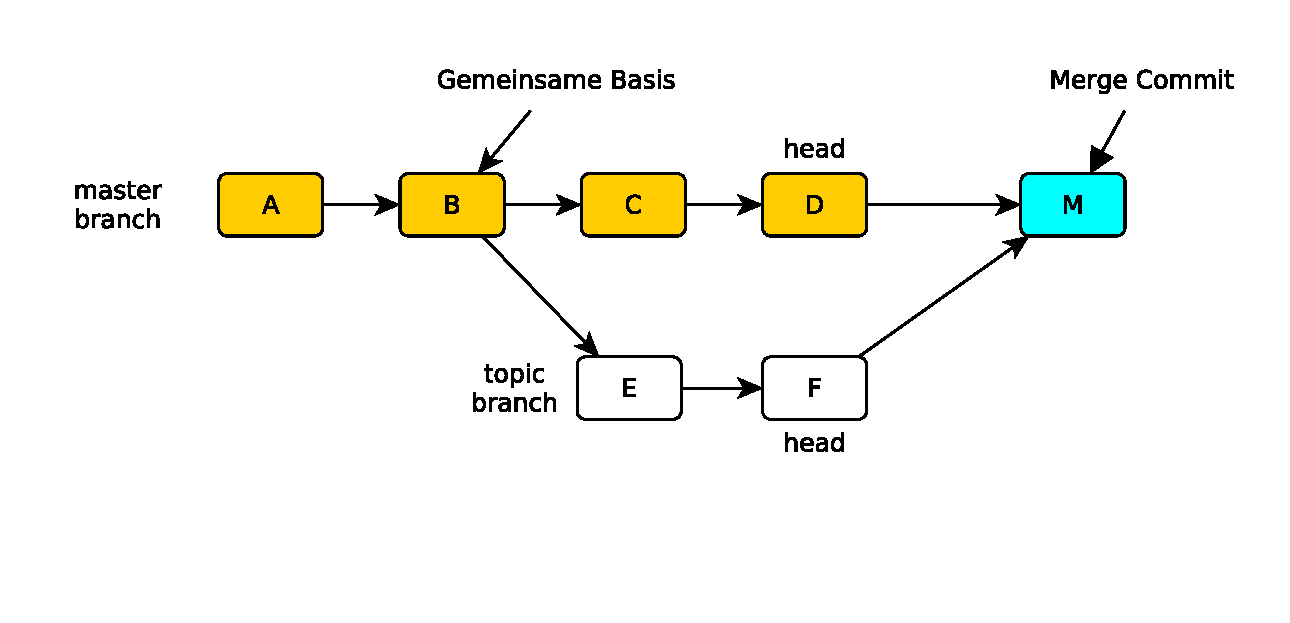
\includegraphics[scale=0.60]{images/merge.eps}
  \caption{Zusammenführen zweier Branches. Angelehnt an \cite[83]{gitosp}}.
  \label{fig:merge}
\end{figure}

Komplexere Szenarien erlauben es, mit Git auch Merges aus mehr als zwei
Branches zu erzeugen, z.B. sogenannte \textit{three-way-merges} oder
\textit{octopus-merges} \cite[S.~87]{gitosp}. Git ermöglicht auch, Zweige aus
verschiedenen Repositorys zusammenzuführen. So gibt es nach \cite[3]{gitwf}
noch die Möglichkeit, Repositorys nach spezielleren Funktionen zu unterteilen.
So kann ein dediziertes \textit{Blessed Repository} ausschließlich für das
Erstellen von Versionen der erzeugten Software genutzt werden. Die Änderungen
können aus einem \textit{Fork Repository} importiert werden. Das \textit{Fork
Repository} dient zur Entkopplung des Haupt-Repositorys. So können größere
Umbauten, Merges oder Features unabhängig vom Haupt-Repository entwickelt
werden \cite[S.~123]{gitwf}. Eine vergleichbare Vorgehensweise findet man im
Repository des Linux Kernels \cite{link:linuxgit} (Abschnitt \ref{sec:kernel}).

\subsection{Repository}\label{sec:repository}
Das Repository ist ein Datenspeicher, in dem gemeinsame Dateien eines Projekts
durch das \acrlong{vcs:de} verwaltet werden. Der Benutzer kann hier Dateien
beispielsweise hinzufügen, entfernen oder verändern und Änderungen in einem
\gls{commit} zusammenfassen. Das \acrlong{vcs:de} erzeugt für alle in
\glspl{commit} zusammengefassten Änderungen eine Historie.
 \cite[S.~38]{hagen:1678}.

\subsection{HEAD}\label{sec:head}
Bei \textit{HEAD} handelt es sich um eine Referenz, die auf den letzten Commit
im aktuellen Repository bzw. Branch verweist. Hier muss zwischen verschiedenen
Versionskontrollsystemen unterschieden werden. So ist unter Git die
\textit{HEAD}\footnote{Git benutzt eine spezielle Syntax für solche Referenzen.
So können Vorgänger (Abschnitt \ref{sec:commitobject}) beispielsweise mit
\texttt{HEAD\^{}} referenziert werden. Das Zeichen \texttt{\^{}} dient dabei
als Zähler. So bezeichntet \texttt{HEAD\^{}\^{}} den zweiten Vorgänger und ist
Aquivalent zu \texttt{HEAD\~{}2}. \cite[S.~65]{gitosp}} Version eine
symbolische Referenz auf die letzte Version des aktuell lokal genutzten
Branches. Diese ist also abhängig von den gerade vorhandenen Daten im Working
Tree von Git \cite[S.~20]{gitosp}. Für \acrshort{svn} hingegen bezeichnet
\textit{HEAD} die letzte veröffentlichte Version im Repository.

\subsection{Checkout}\label{sec:checkout}
Bei vielen Versionskontrollsystemen gibt es einen gleichlautenden Befehl.
Um Missverständnisse zu vermeiden muss man hier zwischen den anderen erwähnten
Versionskontrollsystemen und Git unterscheiden. Der Begriff \textit{checkout}
beschreibt im Rahmen von Versionskonrollsystemen wie z.B. \acrshort{cvs} oder
\acrshort{svn} (Abschnitt \ref{cha:Versionsverwaltung}) das Erstellen einer
lokalen Kopie eines entfernten \glspl{repository} \cite[S~137]{gitosp}.

Im Kontext von Git (Abschnitt \ref{cha:git}) beschreibt \textit{checkout} zum
einen eher das Wechseln zu einem konkreten \gls{commit}. Das kann unter Git ein
\gls{branch}, \gls{tag} oder ein beliebiges Commit-Objekt (Abschnitt
\ref{sec:commit}) sein. Zum anderen können damit auch Dateien aus vorherigen
Commits wiederhergestellt werden \cite[S~76]{gitosp}.

\subsection{Clone}\label{sec:clone}
Was z.B. unter \acrshort{svn} oder \acrshort{cvs} der \textit{checkout} eines
entfernten \glspl{repository} ist, ist unter Git das \textit{Clonen} eines
entfernten \glspl{repository}. Es bezeichnet also das Herunterladen eines
Git-Repositorys von einer Quelle mit der vollständigen Historie und allen
enhaltenen \glspl{commit}. Es erstellt also sozusagen einen Klon des
ursprünglichen \glspl{repository}. \cite[S.~21]{gitosp}

\subsection{Working Tree}\label{sec:workingtree} Es gibt unterschiedliche
Begriffe für den \textit{Working Tree}. So werden synonyme Begriffe wie
Arbeitskopie (engl. \textit{Working Copy}), Arbeitsbereich, \textit{sandbox}
oder auch \textit{checkout} verwendet. Es bezeichnet die gerade aktuelle
Version des lokalen Arbeitsverzeichnisses, an der ggf.  Änderungen vorgenommen
werden können. \cite[S.~20]{gitosp}

\subsection{Index}\label{sec:index}
Der Index ist ein Alleinstellungsmerkmal von Git und bezeichnet eine Ebene
zwischen der Arbeitskopie und dem \gls{repository}. Hier können Änderungen für
einen zukünftigen Commit vorgemerkt werden \cite[S.~20]{gitosp}. Der Index und
dessen Rolle wird im Folgenden nochmal gesondert betrachtet (Abschnitt
\ref{sec:trees}). Dieser Bereich wird häufig auch \textit{Stage} oder
\textit{Staging Area} genannt\cite[S.~11]{progit}.

\section{Arten von Versionsverwaltungssystemen}
\subsection{Lokal}\label{sec:local}
Frühe Versionskontrollsysteme wie \acrshort{rcs} oder \acrshort{cssc} arbeiten
ausschließlich auf dem lokalen Dateisystem und sind nicht dafür entwickelt, ein
kollaboratives Arbeiten zu unterstützen. Der hauptsächliche Anwendungsfall ist,
einem Entwickler eine lokale Versionsverwaltung zu ermöglichen. Die Inhalte
können weiteren Personen nicht mit Mitteln des Versionskontrollsystems zur
Verfügung gestellt werden.

\subsection{Zentral}\label{sec:central}
Versionskontrollsysteme wie \acrshort{svn} oder \acrshort{cvs} stellen ein
zenrales \gls{repository} mit Hilfe einer Serverkomponente zur Verfügung.
Entsprechend dazu gibt es für verschiedene Betriebssysteme Clientkomponenten.
So gibt es für Linux oder andere Unix-Derivate frei verfügbare Server- und
Clientkomponenten, die zum Teil grafisch sowie in einem Terminal zu bedienen
sind. Die Kommunikation der Clientkomponente erfolgt im Regelfall direkt mit
dem Server. Das bedeutet, der Benutzer holt mit dem Client die Dokumente aus
dem zentralen Repository, führt seine Änderungen durch und fasst diese in einem
\gls{commit} zusammen. Hierfür stellt das \acrlong{vcs:de} entsprechende
Unterstützung bereit beispielsweise mit den Befehlen \texttt{checkout}
(Abschnitt \ref{sec:checkout}) zum Holen der Dokumente und
\texttt{commit}(Abschnitt \ref{sec:commit}), zum Zusammenfassen und
gleichzeitigen Übertragen an die Serverkomponente. Die Bearbeitung der
Dokumente im lokalen \gls{repository} erfolgt überwiegend mit unabhängigen
Werkzeugen. \cite[S.~38-40]{hagen:1678}

\subsection{Verteilt}\label{sec:decentral}
Versionskontrollsysteme, die verteilt arbeiten, werden im Englischen
\acrfull{dvcs} genannt und zeichnen sich dadurch aus, dass der Benutzer lokal
ein vollwertiges \gls{repository} zur Verfügung hat, ohne dass eine
Serverkomponente ein zentrales \gls{repository} zur Verfügung stellen muss. Das
ist aber nicht zu verwechseln mit lokalen Versionskontrollsystemen wie
\acrshort{rcs} oder \acrshort{sccs}. Der Unterschied ist, dass verteilte
Systeme das gleichzeitige Arbeiten von mehreren Benutzern stärker unterstützen als
zentrale \acrlong{vcs:de}. Dabei ist es unerheblich, ob Benutzer gleichzeitig
an mehreren Branches, an verschiedenen Repositorys oder an den gleichen
Dateien arbeiten. \cite[S.~393-394]{cd}

Ein Auszug, aus den von Jez Humble und David Farley in \cite[S.~393-394]{cd}
beschriebenen Eigenschaften eines \acrshort{dvcs} lautet wie folgt:

\begin{itemize}
\item Es ist keine Serverkomponente nötig, um einen \gls{commit} in ein lokales
\gls{repository} durchzuführen.
\item \glspl{repository} verschiedener Benutzer und Quellen können miteinander
verbunden werden und deren Inhalte verglichen, integriert oder verändert werden.
\item Um Veränderungen durchzuführen und in einem \gls{commit} zusammenzufassen,
ist es unerheblich, ob eine Netzwerkverbindung zu einer möglichen Quelle besteht.
\item Änderungen können an eingeschränkte Nutzergruppen veröffentlicht werden,
ohne dass jemand gezwungen ist, diese zu übernehmen.
\item Dadurch, dass jeder Benutzer eine eigene vollwertige Kopie des
\glspl{repository} hat, sind \acrshort{dvcs} robuster gegenüber Datenverlusten.
Darüberhinaus können Benutzer dadurch lokal branches anlegen und Experimente
durchführen, ohne diese immer in ein zentrales Repository zu übertragen. Die
geringere Beanspruchung von zentralen Ressourcen, führt zu einer besseren
Skalierbarkeit.
\item Commits, Branches und Tags können lokal sortiert, geordnet und
zusammengefasst werden, bevor die Übertragung in ein gemeinsam genutztes
\gls{repository} durchgeführt wird.\footnote{Das wird im Kontext von Git als
\textit{rebase} bezeichnet.}
\end{itemize}

Im Gegensatz zu zentralen Versionskontrollsystemen erfolgt das Erstellen eines
\glspl{commit} lokal und die Übertragung in ein weiteres \gls{repository}
mit einem zusätzlichen Befehl wie \texttt{push}. Dabei können die Daten beliebig
oft in weitere \glspl{repository} übertragen werden.

\subsection{Streaming}\label{sec:streaming}
Ein populäres Beispiel für ein \acrlong{vcs:de}, das auf Datenströmen
(\textit{Streams}) basiert, ist das kommerziell vermarktete ClearCase von IBM.
Das zentrale Merkmal hierbei ist, dass \textit{Branches} durch sogenannte
Streams ersetzt werden. Das ermöglicht eine Baumstruktur von abhängigen
Zweigen, die durch eine Vererbungsstruktur verbunden sind. Es können Änderungen
innerhalb eines Arbeitsbereichs durchgeführt werden, ohne andere Benutzer zu
beeinflussen. Nach Abschluss dieser Arbeiten können diese veröffentlicht bzw.
\textit{promoted} werden. Diese werden dann allen abhängigen Streams
gleichzeitig zur Verfügung gestellt. Das kann hilfreich sein, um z.B.
grundlegende Softwarebibliotheken auszutauschen oder wichtige Fehlerbehebungen
durchzuführen. In bisher erwähnten Versionskontrollsystemen müssen solche
Änderungen einzeln auf jeden Branch übertragen werden.
